\documentclass[12pt,a4paper]{article}

\usepackage[utf8]{inputenc}
\usepackage[T2A]{fontenc}
\usepackage[ukrainian]{babel}

\usepackage{geometry}
\geometry{left=2cm,right=2cm,top=2cm,bottom=2cm}

\usepackage{graphicx}
\usepackage{array,multirow}
\usepackage{booktabs}
\usepackage{caption}
\renewcommand{\thetable}{№\arabic{table}}
\captionsetup[table]{name=Таблиця}

\usepackage{amsmath}
\usepackage{pdflscape}
\usepackage{xcolor}

\usepackage{hyperref}

\begin{document}

    \begin{titlepage}

        % Картинка шапки (по центру, з відступом від верху)
        \begin{center}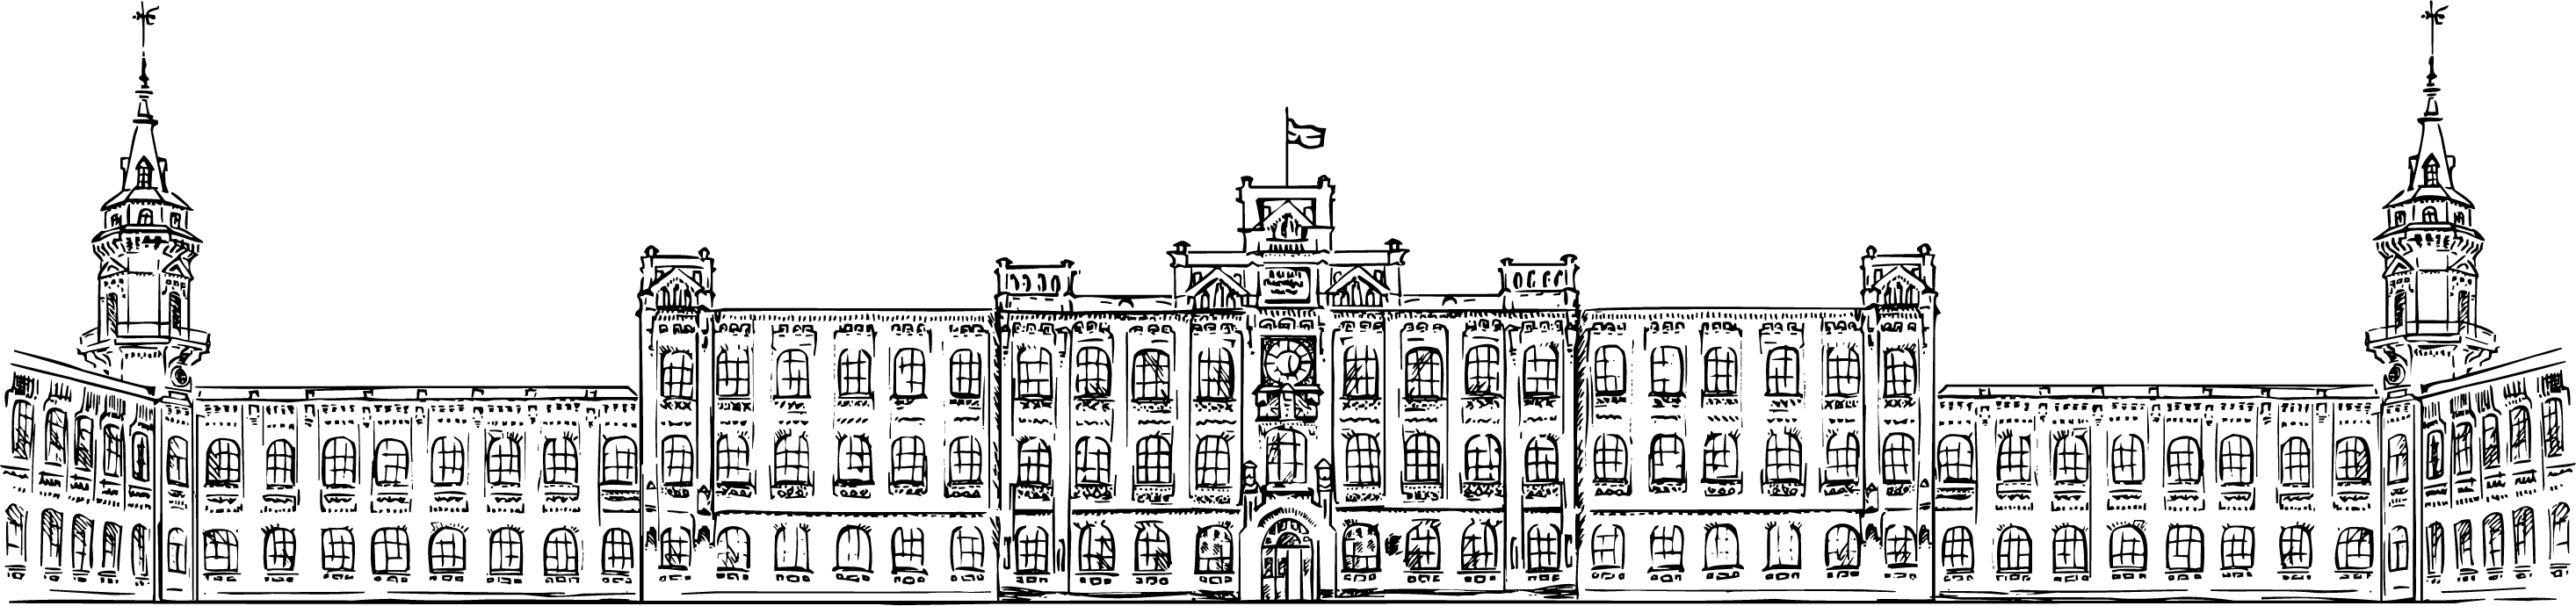
\includegraphics[width=0.7\textwidth]{../../../TITLES/letterhead.png}\end{center}

        \begin{center}
            \large Національний технічний університет України\\
            «Київський політехнічний інститут імені Ігоря Сікорського»\\[1em]
            Факультет інформатики та обчислювальної техніки\\
            Кафедра обчислювальної техніки
        \end{center}

        \vfill

        \begin{center}
            \textbf{\LARGE Психологія конфлікту}\\[2.5em]
            \textbf{\Large Практична робота №1}\\
            «Уявлення про конфлікт у конфліктології»
        \end{center}

        \vfill

        \begin{flushright}
            Виконав: студент 2 курсу ФІОТ, гр. ІО-41\\
            \textit{Давидчук А.~М.}\\[1em]
            Перевірив: \textit{Папуша В.~В.}
        \end{flushright}

        \vfill

        \begin{center}Київ --- 2025\end{center}

    \end{titlepage}

    % Основний документ:

    \section*{Вступ}
    Конфлікт є невід’ємною частиною людського життя та розвитку суспільства. 
    Будь-яке суспільство ґрунтується на різноманітності інтересів, поглядів, цінностей. 
    Коли ці відмінності перетинаються й стають несумісними, виникає конфлікт. 
    Саме тому вивчення закономірностей конфлікту має як теоретичне, так і практичне значення.  

    Конфліктологія як наука оформилася у другій половині XX ст., 
    але її витоки сягають античності: Геракліт стверджував, що боротьба протилежностей 
    є «батьком усього», а Арістотель розглядав конфлікт як загрозу гармонії полісу. 
    У Новий час Томас Гоббс описував людське суспільство як «війну всіх проти всіх», 
    а Карл Маркс визначав соціальні протиріччя рушійною силою історії.  

    \section*{Предмет і завдання конфліктології}
    \textbf{Конфліктологія} — це міждисциплінарна наука, що вивчає закономірності 
    виникнення, розвитку, функціонування та розв’язання конфліктів у різних сферах суспільного життя.

    Основні завдання конфліктології:
    \begin{enumerate}
        \item Дослідження природи й причин виникнення конфліктів.
        \item Аналіз структури та динаміки конфлікту.
        \item Класифікація видів конфліктів.
        \item Розробка стратегій попередження та конструктивного розв’язання.
        \item Формування культури мирного співжиття.
    \end{enumerate}

    \section*{Класифікація конфліктів}
    \textbf{За масштабом:}
    \begin{itemize}
        \item міжособистісні (сім’я, друзі, колеги);
        \item внутрішньоособистісні (боротьба мотивів, когнітивний дисонанс);
        \item групові та організаційні (між підрозділами, колективами);
        \item міждержавні (дипломатичні, військові, економічні).
    \end{itemize}

    \textbf{За змістом:}
    \begin{itemize}
        \item ціннісні (зіткнення переконань, ідеологій, релігійних уявлень);
        \item ресурсні (боротьба за матеріальні чи нематеріальні ресурси);
        \item рольові (конфлікт статусів, очікувань, функцій).
    \end{itemize}

    \textbf{За характером перебігу:}
    \begin{itemize}
        \item відкриті і приховані;
        \item конструктивні (ведуть до розвитку) і деструктивні (руйнують відносини).
    \end{itemize}

    \section*{Структура та динаміка конфлікту}
    Основні елементи:
    \begin{itemize}
        \item \textbf{Сторони конфлікту} — учасники, що мають протилежні інтереси.
        \item \textbf{Предмет конфлікту} — об’єктивна причина протиріч.
        \item \textbf{Образ конфлікту} — уявлення кожної сторони про ситуацію.
        \item \textbf{Інцидент} — подія, що запускає активну фазу.
    \end{itemize}

    \textbf{Динаміка конфлікту:}
    \begin{enumerate}
        \item Накопичення суперечностей (латентна фаза).
        \item Усвідомлення конфлікту сторонами.
        \item Відкрите протистояння.
        \item Ескалація та кульмінація.
        \item Вирішення або згасання конфлікту.
    \end{enumerate}

    \section*{Основні теорії конфлікту}
    \begin{itemize}
        \item \textbf{Діалектична теорія (Гегель, Маркс):} конфлікт — рушійна сила розвитку.
        \item \textbf{Функціоналізм (Парсонс, Мертон):} конфлікт — відхилення від соціальної рівноваги.
        \item \textbf{Льюїс Козер:} конфлікти можуть мати позитивні функції, зокрема інтегрувати групу.
        \item \textbf{Ральф Дарендорф:} конфлікт — наслідок нерівності влади та авторитету.
        \item \textbf{Психологічні теорії:} акцент на особистісних мотивах, емоційних бар’єрах.
    \end{itemize}

    \section*{Методи вирішення конфліктів}
    \begin{itemize}
        \item Переговори — діалог сторін для пошуку спільного рішення.
        \item Посередництво (медіація) — участь третьої нейтральної сторони.
        \item Арбітраж — залучення інституцій чи судових органів.
        \item Компроміс — взаємні поступки.
        \item Консенсус — узгоджене рішення, що задовольняє всіх.
        \item Уникнення чи ігнорування (короткострокова стратегія).
    \end{itemize}

    \section*{Конфлікт як ресурс розвитку}
    Хоча конфлікт часто сприймається негативно, він має і позитивні функції:
    \begin{itemize}
        \item стимулює розвиток організацій та суспільства;
        \item сприяє формуванню нових ідей, інновацій;
        \item допомагає виявити приховані проблеми;
        \item може зміцнювати міжособистісні стосунки після конструктивного розв’язання;
        \item сприяє адаптації системи до змінних умов.
    \end{itemize}

    \section*{Сучасні тенденції}
    У XXI столітті конфліктологія розвивається у кількох напрямах:
    \begin{itemize}
        \item дослідження міжкультурних конфліктів у глобалізованому світі;
        \item вивчення кіберконфліктів та інформаційних війн;
        \item пошук нових методів миротворчості та медіації;
        \item застосування конфліктології у менеджменті, політиці, міжнародних відносинах.
    \end{itemize}

    \section*{Висновки}
    Конфліктологія — це наука, що допомагає зрозуміти неминучість суперечностей 
    і перетворити їх з руйнівної сили на інструмент розвитку. 
    Вона формує культуру конструктивного спілкування, 
    розвиває навички ведення переговорів і дозволяє знаходити рішення, 
    які сприяють гармонії та прогресу в суспільстві.

\end{document}